%%%%%%%%%%%%%%%%%%%%%%%%%%%%%%%%%%%%%%%%%
% Masters/Doctoral Thesis 
% LaTeX Template
% Version 2.5 (27/8/17)
%
% This template was downloaded from:
% http://www.LaTeXTemplates.com
%
% Version 2.x major modifications by:
% Vel (vel@latextemplates.com)
%
% This template is based on a template by:
% Steve Gunn (http://users.ecs.soton.ac.uk/srg/softwaretools/document/templates/)
% Sunil Patel (http://www.sunilpatel.co.uk/thesis-template/)
%
% Template license:
% CC BY-NC-SA 3.0 (http://creativecommons.org/licenses/by-nc-sa/3.0/)
%
%%%%%%%%%%%%%%%%%%%%%%%%%%%%%%%%%%%%%%%%%

%----------------------------------------------------------------------------------------
%	PACKAGES AND OTHER DOCUMENT CONFIGURATIONS
%----------------------------------------------------------------------------------------
\documentclass[
11pt, % The default document font size, options: 10pt, 11pt, 12pt
oneside, % Two side (alternating margins) for binding by default, uncomment to switch to one side
english, % ngerman for German
singlespacing, % Single line spacing, alternatives: onehalfspacing or doublespacing
%draft, % Uncomment to enable draft mode (no pictures, no links, overfull hboxes indicated)
%nolistspacing, % If the document is onehalfspacing or doublespacing, uncomment this to set spacing in lists to single
%liststotoc, % Uncomment to add the list of figures/tables/etc to the table of contents
%toctotoc, % Uncomment to add the main table of contents to the table of contents
%parskip, % Uncomment to add space between paragraphs
%nohyperref, % Uncomment to not load the hyperref package
headsepline, % Uncomment to get a line under the header
chapterinoneline, % Uncomment to place the chapter title next to the number on one line
%consistentlayout, % Uncomment to change the layout of the declaration, abstract and acknowledgements pages to match the default layout
]{MastersDoctoralThesis} % The class file specifying the document structure

\usepackage[utf8]{inputenc} % Required for inputting international characters
\usepackage[T1]{fontenc} % Output font encoding for international characters
\usepackage{mathpazo} % Use the Palatino font by default
\usepackage{cite}

%\usepackage[backend=bibtex,style=numeric,sorting=none, maxbibnames=99]{biblatex} % Use the bibtex backend with the authoryear citation style (which resembles APA)

%\addbibresource{~/BibTex/BibTex.bib} % The filename of the bibliography

\usepackage[autostyle=true]{csquotes} % Required to generate language-dependent quotes in the bibliography

\usepackage{amstext, amsfonts, amsmath, amsbsy, amssymb}
\usepackage{tikz}
\usepackage{booktabs}
\usepackage{pgfplots}
\usepackage{caption}
\usepackage{subcaption}
\usepackage{easyReview}

%----------------------------------------------------------------------------------------
%	MARGIN SETTINGS
%----------------------------------------------------------------------------------------

\geometry{
	paper=a4paper, % Change to letterpaper for US letter
	inner=2.5cm, % Inner margin
	outer=3.8cm, % Outer margin
	bindingoffset=.5cm, % Binding offset
	top=1.5cm, % Top margin
	bottom=1.5cm, % Bottom margin
	%showframe, % Uncomment to show how the type block is set on the page
}

%----------------------------------------------------------------------------------------
%	THESIS INFORMATION
%----------------------------------------------------------------------------------------

\thesistitle{ACOL : Random Markov Field} % Your thesis title, this is used in the title and abstract, print it elsewhere with \ttitle
\supervisor{Prof. Daniel \textsc{Wegmann} \\ \& Dr. Pierre-Marie \textsc{Allard}} % Your supervisor's name, this is used in the title page, print it elsewhere with \supname
\examiner{} % Your examiner's name, this is not currently used anywhere in the template, print it elsewhere with \examname
\degree{Master of Science in Bioinformatics and Computational Biology} % Your degree name, this is used in the title page and abstract, print it elsewhere with \degreename
\author{Marco \textsc{Visani}} % Your name, this is used in the title page and abstract, print it elsewhere with \authorname
\addresses{} % Your address, this is not currently used anywhere in the template, print it elsewhere with \addressname

\subject{Biological Sciences} % Your subject area, this is not currently used anywhere in the template, print it elsewhere with \subjectname
\keywords{} % Keywords for your thesis, this is not currently used anywhere in the template, print it elsewhere with \keywordnames
\university{\href{https://www.unifr.ch/}{University of Fribourg}} % Your university's name and URL, this is used in the title page and abstract, print it elsewhere with \univname
\department{\href{https://www.unifr.ch/bio/en/}{Department of Biology}} % Your department's name and URL, this is used in the title page and abstract, print it elsewhere with \deptname
\group{\href{https://www.unifr.ch/bio/en/groups/wegmann/}{Wegmann Group} \& \href{https://www.unifr.ch/bio/en/groups/allard/}{COMMONS Lab}} % Your research group's name and URL, this is used in the title page, print it elsewhere with \groupname
\faculty{\href{https://www.unifr.ch/scimed/en/}{Faculty of Science and Medicine}} % Your faculty's name and URL, this is used in the title page and abstract, print it elsewhere with \facname

\AtBeginDocument{
\hypersetup{pdftitle=\ttitle} % Set the PDF's title to your title
\hypersetup{pdfauthor=\authorname} % Set the PDF's author to your name
\hypersetup{pdfkeywords=\keywordnames} % Set the PDF's keywords to your keywords
}


%----------------------------------------------------------------------------------------
%	MATH STUFF
\usepackage{amstext, amsfonts, amsmath, amsbsy, amssymb}
\DeclareMathOperator{\Poisson}{Poisson}
\DeclareMathOperator{\Multinom}{Multinom}
\DeclareMathOperator{\logit}{logit}
\DeclareMathOperator{\cov}{cov}
\DeclareMathOperator{\Ind}{I}
\def\P{\mathbb{P}}
\def\E{\mathbb{E}}

\def\x{\boldsymbol{x}}

\def\btau{\boldsymbol{\tau}}
\def\bmu{\boldsymbol{\mu}}
\def\bxi{\boldsymbol{\xi}}
\def\bLambda{\boldsymbol{\Lambda}}
\def\bP{\boldsymbol{P}}
\def\bd{\boldsymbol{d}}


\def\Ccal{{\cal C}}
\def\C{{\cal C}}
\def\E{{\cal E}}
\def\I{{\cal I}}
\def\N{{\cal N}}
\def\M{{\cal M}}
\def\R{{\cal R}}
\def\T{{\cal T}}
\def\X{{\cal X}}
\def\Y{{\cal Y}}
\def\Z{{\cal Z}}
\def\D{{\cal D}}


%----------------------------------------------------------------------------------------

\linespread{1.25}
\begin{document}


\frontmatter % Use roman page numbering style (i, ii, iii, iv...) for the pre-content pages

\pagestyle{plain} % Default to the plain heading style until the thesis style is called for the body content

%----------------------------------------------------------------------------------------
%	TITLE PAGE
%----------------------------------------------------------------------------------------

\begin{titlepage}

\includegraphics[scale=0.3]{images/UnifrLogo} % University logo
\begin{center}
\vspace*{.06\textheight}
{\scshape\LARGE \univname\par}\vspace{1.5cm} % University name

\textsc{\Large Manuscript}\\[0.5cm] % Thesis type

\HRule \\[0.4cm] % Horizontal line
{\huge \bfseries \ttitle\par}\vspace{0.4cm} % Thesis title
\HRule \\[1.5cm] % Horizontal line
 
\begin{minipage}[t]{0.4\textwidth}
\begin{flushleft} \large
\emph{Authors:}\\
\href{mailto:madleina.caduff@unifr.ch}{Madleina \textsc{Caduff}}\\
\href{mailto:contact@vismarco.ch}{\authorname} % Author name - remove the \href bracket to remove the link
\end{flushleft}
\end{minipage}
\begin{minipage}[t]{0.4\textwidth}
\begin{flushright} \large
\emph{Supervisors:} \\
\href{mailto:daniel.wegmann@unifr.ch}{Prof. Daniel \textsc{Wegmann}} \\
\href{mailto:pierre-marie.allard@unifr.ch}{Dr. Pierre-Marie \textsc{Allard}}% Supervisor name - remove the \href bracket to remove the link  
\end{flushright}
\end{minipage}\\[3cm]
 
\vfill

%\large \textit{A thesis submitted in fulfillment of the requirements \\ for the degree of \degreename}\\[0.3cm] % University requirement text
%\textit{in the}\\[0.4cm]
%\groupname\\\deptname\\[2cm] % Research group name and department name
 
\vfill

{\large \today}\\[4cm] % Date
%\includegraphics{Logo} % University/department logo - uncomment to place it
 
\vfill
\end{center}
\end{titlepage}

%----------------------------------------------------------------------------------------
%	LIST OF CONTENTS/FIGURES/TABLES PAGES
%----------------------------------------------------------------------------------------

\tableofcontents % Prints the main table of contents

%\listoffigures % Prints the list of figures

%\listoftables  % Prints the list of tables

%----------------------------------------------------------------------------------------
%	ABBREVIATIONS
%----------------------------------------------------------------------------------------
%
\begin{abbreviations}{ll}\label{sec:abbreviations} % Include a list of abbreviations (a table of two columns)
	
\textbf{DAG} & \textbf{D}irected \textbf{A}cyclic \textbf{G}raph\\
\textbf{GNN(s)} & \textbf{G}raph \textbf{N}eural \textbf{N}etwork(s) \\
\textbf{MS} & \textbf{M}ass \textbf{S}pectrometry \\
\textbf{NP(s)} & \textbf{N}atural \textbf{P}roduct(s) \\
\textbf{RMF} & \textbf{R}andom \textbf{M}arkov \textbf{F}ield \\



\end{abbreviations}


%----------------------------------------------------------------------------------------
%	THESIS CONTENT - CHAPTERS
%----------------------------------------------------------------------------------------

\mainmatter % Begin numeric (1,2,3...) page numbering

\pagestyle{thesis} % Return the page headers back to the "thesis" style

% Include the chapters of the thesis as separate files from the Chapters folder
% Uncomment the lines as you write the chapters

%\include{Chapters/1_introduction}
%\include{Chapters/2_litterature_review} 
%\include{Chapters/3_methods}
%\include{Chapters/4_results} 
%\include{Chapters/5_discussion} 
%\include{Chapters/6_conclusion}

\chapter{Random Markov Field}
\section{Detailed Research Plan}
We seek to infer the presence or absence of NPs in a group of samples compartmentalized by several discrete dimensions such as \textit{e.g.} species, tissue or environmental conditions. We assume that the pattern of presence and absence is modulated by similarities within each dimension. For instance, closely related species may share a similar set of NPs and NPs related in their synthesis may share a similar distribution across species. To model such similarities, we adopt a \href{https://en.wikipedia.org/wiki/Markov_random_field}{Markov Random Field} (MRF) approach.

Let $D\geq2$ denote the total number of dimensions, of which, without loss of generality, the first shall be the NP and the second the species. Each dimension $d=1, \ldots, D$ consist of a set $\E_d$ of discrete entries (e.g. individual species along the species dimension). We model similarities between the entries of dimension $d$ using a Markov process along a known tree $\T_d$ consisting of $\N_d = \E_d \cup \R_d \cup \I_d$ nodes: the entries $\E_d$ are leaves, connected to the set of roots $\R_d$ through a set of internal nodes $\I_d$. For every node $n \in \N_d, n \notin \R_d$ that is not a root, let $p(n) \in \N_d$ denote its parent node and $b(n) \geq 0$ the length of the branch connecting it to its parent (see Figure \ref{fig:method-overview}A for an example).

\paragraph{Markov Random Field} Let $\X$ denote a Markov Random Field of which each variable $x \in \X$ represents a combination of nodes from each of the $D$ dimensions and indicates the presence ($x=1$) or absence ($x=0$) of the NP for that combination of nodes (see Figure \ref{fig:method-overview}A for an example with two dimensions). Let $\delta_d(x) \in \N_d$ reflect the node of $x$ in dimension $d$ with $\delta_1(x)$ indicating the NP of $x$, and let $\delta(x)=(\delta_1(x), \ldots, \delta_D(x))$ be the vector of nodes across all dimension $D$. We only consider two sets of variables: 1) the set $\Y$ of variables representing a leaf in each dimension such that for a variable $y\in\Y$, $\delta_d(y) \in \E_d$ for all $d=1, \ldots, D$, and 2) the set $\Z$ of variables representing leaves in all dimensions except one such that for a variable $z \in \Z$, $\delta_k(z) \in \I_k$ and $\delta_d(z) \in \E_d$ for all $d \neq k$. We then have $\X = \Y \cup \Z$ and $\Y \cap \Z = \varnothing$.


We suppose that the joint density of $\X$ can be factorized over a set of \href{https://en.wikipedia.org/wiki/Clique_(graph_theory)}{cliques} $\C$. Each clique $c \in \C$ consists of a set of variables of $\X$ that represent the same leaves in all but one dimension $k$. Specifically, for all $x,x' \in c$, $\delta_k(x) \in \N_k$, $\delta_{d \neq k}(x) = \delta_d(x') \in \E_d$ (see Figure \ref{fig:method-overview}A for an illustration). For such a clique, we will refer to the dimension $\nu(c) = k$ as its \emph{variable} dimension and will denote by $\delta_{-\nu(c)}(c)$ the vector of nodes in the \emph{fixed} dimensions. By definition, $\delta_{-\nu(c)}(c)=\delta_{-\nu(c)}(x)$ for every $x \in c$.

We will further denote by $\C_k \subset \C$ the subset of cliques that share the variable dimension $k$, \textit{i.e.} $\nu(c)=k$ for all $c \in \C_k$. Note that each clique is in exactly one subset ($\C_k \cap \C_d = \varnothing$ for all $k \neq d$) and cliques of the same subset do not share any variables ($c_1 \cap c_2 = \varnothing$ for all $c_1, c_2 \in C_k$). However, each variable $x \in \Y$ will be part of exactly one clique from each subset: the clique $c \in \C_k$ for which $\delta_{-k}(c) = \delta_{-k}(x)$. In contrast, each variable $x \in \Z$ will be part of exactly one clique: the clique $c \in \C$ for which $\delta_{-\nu(c)}(c) = \delta_{-\nu(c)}(x)$ and $\delta_{\nu(c)}(x) \in \I_{\nu(c)}$.


The joint density of $\X$ factorizes as
\begin{equation}
	\P(\X) = \prod_{d=1}^D \prod_{c \in \C_d} \phi(c).
\end{equation}

\paragraph{Markov model along trees} We will model the clique functions $\phi(c)$ using a Markov model along tree $\T_d$. Let
\begin{equation}
	\bLambda_c =
	\begin{pmatrix}
		-\mu_{c1} & \mu_{c1}\\
		\mu_{c0} & -\mu_{c0}\\
	\end{pmatrix}
\end{equation}
be the rate matrix for changes between states 0 and 1 along the tree. For each node $n \in \N_d, n \notin \R_d$ that is not a root, the transition probabilities between parent node $p(n)$ and $n$ are then given by
\begin{equation}
	\bP(n) = \exp(\bLambda_c b(n)).
\end{equation}

We assume the root state probabilities are given by the stationary distribution of the Markov chain:
\begin{equation}
	\bP_{\infty} = \left(\frac{\mu_{c0}}{\mu_{c0} + \mu_{c1}}, \frac{\mu_{c1}}{\mu_{c0} + \mu_{c1}}\right).
\end{equation}


The clique function $\phi(c)$ is given by
\begin{equation}
	\phi(c) = \prod_{x \in c, }\Big( \Ind(x \in \R_{\nu(c)})[\bP_{\infty}]_x\\
	+ \Ind(x \notin \R_{\nu(c)}) [\bP(\delta_{\nu(c)}(x))]_{p_{c}(x), x} \Big)
\end{equation}

where we used the shorthand $x \in \R_{\nu(c)}$ for $\delta_{\nu(c)}(x) \in \R_{\nu(c)}$ to indicate whether the node in the variable dimension of $c$ of $x$ is a root and $p_{c}(x)$ to identify the variable $z \in c$ for which $\delta_{\nu(c)}(z) = p(\delta_{\nu(c)}(x))$.


\paragraph{Inference \& Scalability}

The number of species and NPs in nature are huge. The model proposed above was carefully crafted to scale to these numbers. The total number of hierarchical parameters to infer are two rate parameters per clique and one branch length per node of each dimension, regardless of the number or size of the other dimensions. We will infer all parameters under a Bayesian scheme using Markov Chain Monte Carlo (\href{https://en.wikipedia.org/wiki/Markov_chain_Monte_Carlo}{MCMC}) techniques to obtain posterior probabilities on all $x \in \X$.

\subsubsection{Observed data}

We consider two types of data to inform about $\X$:  i) presence-only reports of specific NPs in specific species as available through the LOTUS database \cite{rutz_2022a} and ii) presence-absence data obtained with mass-spectrometry (LC-MSMS). We outline emission models for both types of data, but stress that these are mere starting points and may be made more elaborate in the future.

\paragraph{LOTUS }

Let $L_{ms} = 1$ denote a known occurrence of NP $m$ in species $s$, and let $L_{ms}=0$ denote that no evidence for such an occurrence has been reported, either because the NP $m$ is truly absent in species $s$ or because of a lack of research effort.

Let $x(m,s)$ denote the variable in $\X$ for NP $m$ and species $s$, which, in case $\X$ contains additional dimensions, is obtained by collapsing:
\begin{equation*}
	x(m,s) = \min \left(1, \sum_{x \in \X} \Ind(\delta_1(x)=m) \Ind(\delta_2(x)=s) x \right).
\end{equation*}

We will model the probability of $L_{ms}$ given $x(m,s)$ as a function of $R_{sm}$, the probability of discovery of NP $m$ in species $s$, such that
\begin{equation*}
	\P(L_{ms}|\x(m,s), R_{ms}) =
	\begin{cases}
		0 \quad &\mathrm{if\ } \x(m,s)=0, L_{ms} = 1,\\
		1 \quad &\mathrm{if\ } \x(m,s)=0, L_{ms} = 0,\\
		R_{ms} \quad &\mathrm{if\ } \x(m,s)=1, L_{ms} = 1,\\
		1- R_{ms} \quad &\mathrm{if\ } \x(m,s)=1, L_{ms} = 0.
	\end{cases}
\end{equation*}

The probability of discovery $R_{ms}$ will be modeled as a function of the known total number of relevant papers published for NP $m$ ($P_m$) and for species $s$ ($Q_s$), such that
\begin{equation*}
	R_{ms} = 1 - e^{-\gamma P_m - \delta Q_s}
\end{equation*}
with positives scalars $\gamma$ and $\delta$ that we will infer.

\paragraph{LC-MSMS}\label{sec:ModellingLCMS}

\begin{figure}
	\centering
	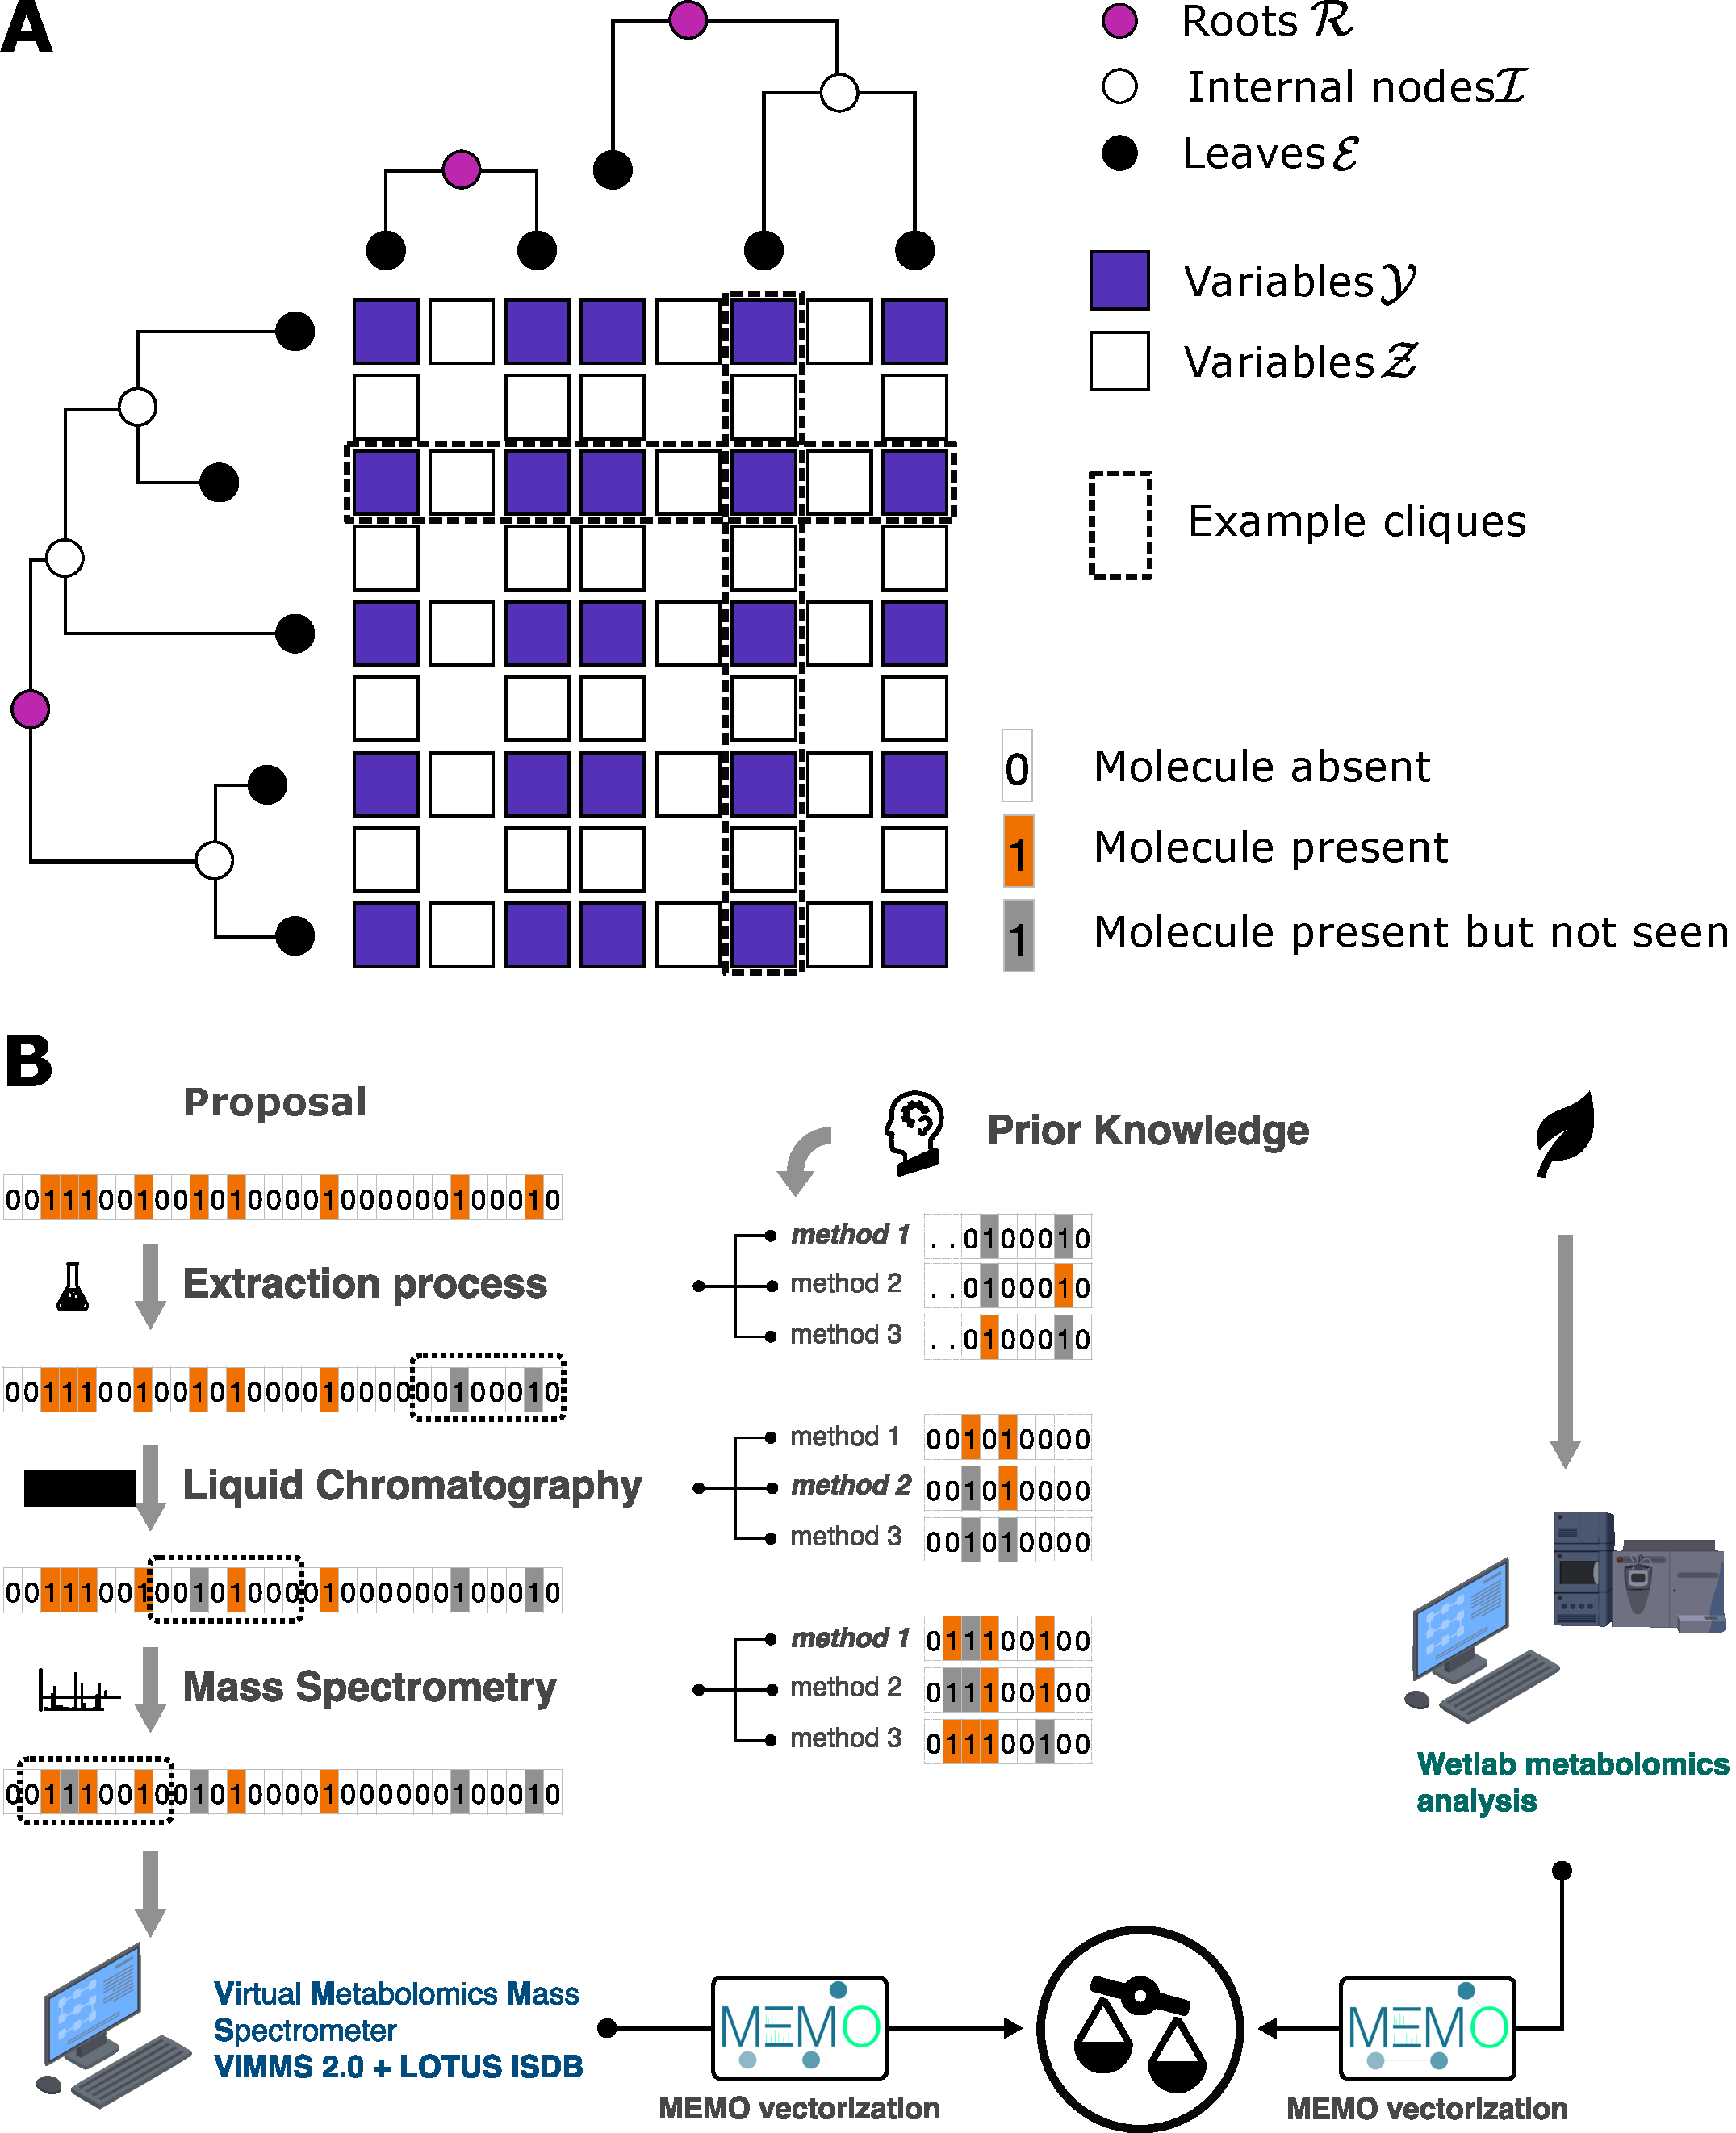
\includegraphics[width=0.45\textwidth]{./images/method_figure_complete_vertical.pdf}
	\caption{Visualizations of core models. A) An illustration of a Markov Random Field for two dimensions (\textit{e.g.} NPs and species). B) Workflow to calculate the probability of the observed mass-spectrometry data given a proposed vector indicating the presence of NPs in a species. \href{https://commons-research.github.io/snf-anticipating-the-chemistry-of-life/method_figure_complete_vertical.pdf}{Full figure here}.}
	\label{fig:method-overview}
\end{figure}


Ultra High Performance Liquid Chromatography coupled to fragmentation Mass Spectrometry (LC-MSMS) is the analytical workhorse for the molecular characterization of complex biological matrices. Coupled to computational mass spectrometry tools, such untargeted approaches allows to detect and putatively annotate thousands of NPs in a single run. These analysis are fundamental in our project as they will allow us to complete the currently patchy overview offered by LOTUS. However, the resulting data is complex and requires careful processing to be informative as it is high-dimensional, noisy and incomplete. We here propose a model that builds on previous work regarding the Liquid Chromatography (LC) process \cite{heymann_2023,wiczling_2021}, the establishment of virtual mass spectrometers \cite{wandy_2019,wandy_2022,wandy_2023} and the integration of LC and MS dimensions in the NP annotation process \cite{bach_2021, bach_2022}, yet is simpler and more streamlined to render it computationally feasible for the large scales considered here.

Suppose $\D_i$ is an LC-MSMS profile obtained from a sample representing a specific vector $\bxi=(\xi_{i2}, \ldots, \xi_i{D}), \xi_{id} \in \E_d$ of leaves in all dimensions except NPs one, such as, for instance, a sample representing a specific tissue of a specific species. We will calculate the probability of the LC-MSMS data $\D_i$ given $\X$ as schematized in Figure \ref{fig:method-overview}B: Let $\x(\bxi_i) \subset \X$ denote a slice through $\X$ relevant for $\D_i$, \textit{i.e.} consisting of all variables that represent a leave in the metabolite dimension and the specific leaves $\bxi$ in each other dimension such that for all $x,x' \in \x(\bxi_i)$, $\delta_1(x) \in \N_1$, $\delta_1(x) \neq \delta_1(x')$ and $\delta_{d \neq 1}(x) =\delta_{d \neq 1}(x') = \xi_{id} \in \E_d$. We will develop an NPs-flavored \textbf{Vi}rtual \textbf{M}etabolomics \textbf{M}ass \textbf{S}pectrometer (\textbf{ViMMS}) building on the original implementation \cite{wandy_2019}. It will be fed by an in silico spectral database of the last LOTUS contents (\href{https://doi.org/10.5281/zenodo.8287341}{ISDB-LOTUS}) and informed by prior expert knowledge regarding the classes of analytes lost in the reductionist and stochastic metabolomics approach here formed by \textit{extraction}, \textit{liquid chromatography} and \textit{mass spectrometry fragmentation} stages. The NPs-ViMMS will allow the generation of theoretical metabolomics datasets for any given input ($\D_i'$), these will be then be compared to experimental results ($\D_i$).

To compare the resulting LC-MSMS profile $\D_i'$ to $\D_i$, we will then take advantage of \textbf{MEMO} (MS2 BasEd SaMple VectOrization), a method we recently established for the computationally efficient comparison of large sets of samples based on their LC-MSMS profiles \cite{gaudry_2022}. The first step is to extract fragment ions and neutral losses from each MSMS spectrum binned from the detected features in so-called “documents” using Spec2Vec \cite{huber_2021}. Then, for a given sample, all the documents created are aggregated based on word occurrences to form a fingerprint (a MEMO vector). The MEMO strategy exploits the advantages of LC, namely its separation power (thus simplifying the chemical complexity of the sample being analyzed and allowing resolution of isomerisms) while avoiding the disadvantages of RT-based alignment since MEMO vectors contain only mass spectrometry information. Here we'll implement a stochastic comparison of MEMO vectors $\M(\D_i')$ and $\M(\D_i)$ using a per entry error rate $\epsilon$ to be inferred from the data. 

%----------------------------------------------------------------------------------------
%	THESIS CONTENT - APPENDICES
%----------------------------------------------------------------------------------------

\appendix % Cue to tell LaTeX that the following "chapters" are Appendices

% Include the appendices of the thesis as separate files from the Appendices folder
% Uncomment the lines as you write the Appendices

%\include{Appendices/AppendixA}
%\include{Appendices/AppendixB}
%\include{Appendices/AppendixC}

%----------------------------------------------------------------------------------------
%	BIBLIOGRAPHY
%----------------------------------------------------------------------------------------
%\printbibliography
\renewcommand{\bibname}{References}
\bibliographystyle{unsrturl}
\bibliography{manuscript}


%----------------------------------------------------------------------------------------

\end{document}  
